%%%%%%%%%%%%%%%%%%%%%%%%%%%%%%%%%%%%%%%%%%%%%
% ELO 2,3,5,6
% Planning for Detailed Design

% Chapter 4: Detailed Design

% System Diagram with functional blocks 

% 4.1 Detailed design of component 1
% I chose to use a Mongo database instead of {x,y,z} because of ...
% List technical details

% 4.2 Detailed design of component 2

% 4.3 Detailed design of component 3

% 4.4 Detailed design of component 4v
%%%%%%%%%%%%%%%%%%%%%%%%%%%%%%%%%%%%%%%%%%%%%

\chapter{Low-Level System Design} 
\label{Detailed_design}

%\begin{figure}[H]
%    \centering
%    \includegraphics[scale=1]{Figures/Goal4.png}
%    \caption{Logical inference in context}
%    \label{fig:python_implment}
%\end{figure}	


\section{Detailed sub-systems descriptions}
%In my case this will be code design like in E-Design.
%Mirror the functional blocks.
%In depth calculations or mathematical representation.
%\subsection{Agent}
%\begin{algorithm}[H]
%\SetAlgoLined
%\KwResult{Add states and actions to knowledge base}
%	\Indp
%	\textbf{Begin} Executor class \\
%	$\phi(x)=\pi$\\
%	$\int_{a}^{b} \phi(x) dx=\pi[b-a]$\\
%	\textbf{End} Executor class
%  \Indm adasd 
% \caption{Agent Algorithm}
%\end{algorithm}



\subsection{Environment}
\subsection{Knowledge Base}
\subsection{Inference Procedure}




\section{Learning Algorithms} 
\section{Forming groups of states}
\subsection{Split state definitions using AND}
\subsection{Merge state definitions using OR}
%\citep{Discrete_Maths}
\newpage
\subsection{Program Flow}
\begin{figure}[H]
    \centering
    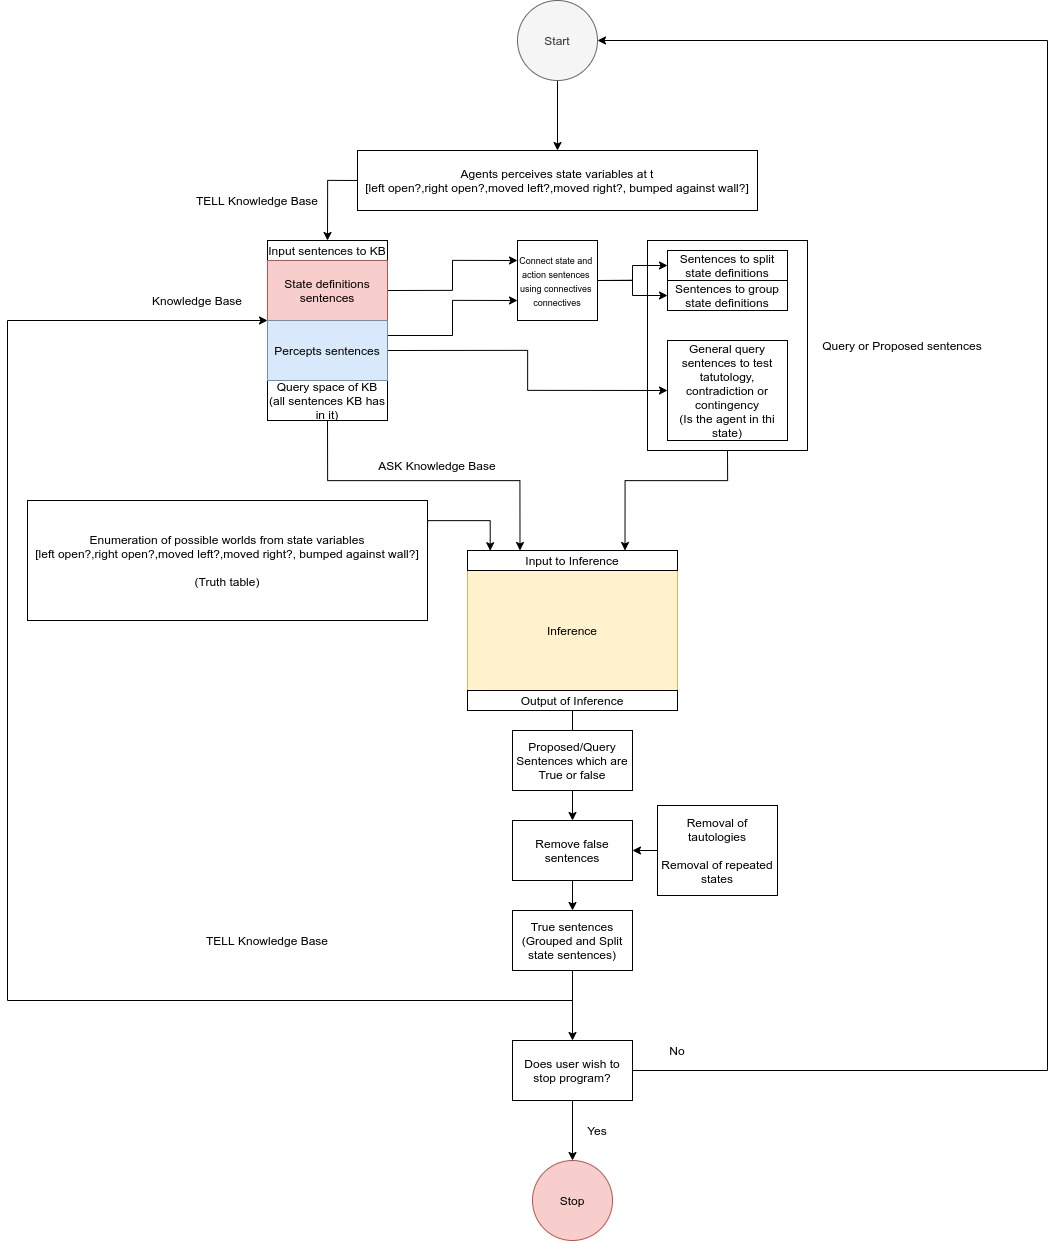
\includegraphics[scale=.4]{Figures/new_program_flow.jpg}
    \caption{Program Flow for full system} 
    \label{fig:program_flow}
\end{figure}